\documentclass[preprint,12pt]{elsarticle}
% Manuscript of the study in this repository (Brief 20, Part M). Every number in the text is traced to a numbers or
% results file by manuscript/numbers_check.py; the figures are built by src/make_manuscript_figures.py and the tables
% by src/make_manuscript_tables.py from the results files.
\usepackage[T1]{fontenc}
\usepackage{amsmath}
\usepackage{graphicx}
\usepackage{booktabs}
\usepackage{lineno}
\usepackage{textcomp}
\usepackage[hidelinks]{hyperref}
\usepackage{xcolor}
\newcommand{\degC}{\,\textdegree C}
\newcommand{\fs}{f^{*}}
\newcommand{\ft}{f_{\mathrm{t}}}
\newcommand{\fmax}{f_{\mathrm{max}}}
\newcommand{\Eb}{E_{\mathrm{b}}}
\newcommand{\Ee}{E_{\mathrm{e}}}
\newcommand{\PH}[1]{\textcolor{red}{[#1]}}
\biboptions{sort&compress}
\journal{Journal of Power Sources}

\begin{document}

\begin{frontmatter}

\title{Neither conduction nor a fixed delivered energy fraction reproduces sixteen two-cell propagation tests: a pre-registered kinetic study}

\author{Siddharth Satte}
% The corresponding author's e-mail address is added at submission; it is not committed to the public repository.
\address{Independent researcher, Pune, India}

\begin{abstract}
%ABSTRACT-START
\PH{abstract, written after Stage 11}
%ABSTRACT-END
\end{abstract}

\begin{keyword}
Thermal runaway propagation \sep Lithium-ion battery \sep Decomposition kinetics \sep Bayesian chemical reaction neural network \sep Two-cell test \sep Pre-registration \sep LG M50
\end{keyword}

\end{frontmatter}

\linenumbers

%BODY-START
\section{Introduction}
\label{sec:intro}

\PH{introduction, written with the verified references}

\section{Methods}
\label{sec:methods}

The study ran in eleven stages. Each stage's predictions, with the expectation held for each, were committed to a public repository and pushed before any of its runs, and the stage's inputs were recorded in a decisions log before they were used; Section~\ref{sec:prereg} gives the record. The methods below are those of the stages whose results this paper reports, in the order of the claims.

\subsection{Two cells, two neighbours}
\label{sec:geometry}

The geometry is that of a published two-cell study~\cite{Satte2026twocell}: two LG M50 cylindrical cells (21700 format, 21.1~mm in diameter and 70.1~mm long) side by side with parallel axes (Fig.~\ref{fig:geometry}a). The trigger (cell~1) is one temperature, which releases its body energy $\Eb$ inside itself as a triangular pulse. The neighbour (cell~2) is solved twice from the same history of the trigger: as one temperature, the lumped neighbour, and as a three-dimensional field, the resolved neighbour, a half model on 19,355 nodes with its symmetry plane through both axes. The resolved roll conducts 1.3~W\,m$^{-1}$\,K$^{-1}$ across its layers and 25~W\,m$^{-1}$\,K$^{-1}$ along them, inside a 0.25~mm steel can; both neighbours hold the cell's heat capacity, 61.75~J\,K$^{-1}$. In Stages~1 to 4 the cells stand 2~mm apart joined by busbars, as the two-cell study archived them: Stage~1 integrates the kinetics along its archived temperature histories, Stage~2 feeds their heat back into both solvers (one-way), and Stages~3 and 4 repeat Stage~1 over the posterior. From Stage~5 on, the cans touch along a line, as in the tests~\cite{Fransson2024}. Within 45\textdegree{} of the line of contact the conductance per unit area is a steel-on-steel contact conductance $h_c$ in series with the air wedge, $h(\theta)=k_{\mathrm{air}}/(\delta(\theta)+k_{\mathrm{air}}/h_c)$ with $\delta=2R(1-\cos\theta)$, and $h_c$ is 200, 2,000 or 3,700~W\,m$^{-2}$\,K$^{-1}$ for the low, central and high contact~\cite{Lienhard2020}; nickel-strip tabs join the cells (5, 6.8 and 10~mW\,K$^{-1}$ each, one in series and two in parallel)~\cite{Satte2026twocell}; the cans radiate to each other (view factor 0.1817~\cite{Incropera2007}) and to the room, and lose heat to it by convection, at 25\degC. The hot spot is the resolved neighbour's hottest node at each time; the far face is the surface node at mid-length opposite the line of contact. A step splits the reaction, integrated node by node, from the backward-Euler conduction step, at a length that keeps any node's reaction heating within 1~K a step. Table~\ref{tab:params} lists the parameters and their sources.

\begin{table}[p]
\centering
\scriptsize
\caption{The model's parameters and their sources: a published source, the two-cell study whose geometry and solver this study takes~\cite{satte2026twocell}, or an entry of this study's decisions log (D, in the repository~\cite{satte2026repo}). Values in parentheses are brackets run as sensitivities or the ranges of the thermal draws.}
\label{tab:params}
\renewcommand{\arraystretch}{0.92}
\begin{tabular}{p{0.29\textwidth}p{0.37\textwidth}p{0.24\textwidth}}
\toprule
Quantity & Value & Source \\
\midrule
\multicolumn{3}{l}{\textit{Geometry}} \\
Cell diameter and length & 21.1 and 70.1 mm & two-cell study~\cite{satte2026twocell} \\
Can: wall, conductivity; mass and specific heat & 0.25 mm, 15 W\,m$^{-1}$\,K$^{-1}$; 9 g, 500 J\,kg$^{-1}$\,K$^{-1}$ & two-cell study~\cite{satte2026twocell} \\
Resolved neighbour & half model, 19,355 nodes (145,195 halved) & this study (D42) \\
\multicolumn{3}{l}{\textit{Thermal properties}} \\
Roll conductivity, across and along the layers & 1.3 and 25 W\,m$^{-1}$\,K$^{-1}$ (draws 0.998 to 1.38; 24.9 to 25.8) & \cite{oregan2022thermal,chen2021simplified}; D27 \\
Cell heat capacity & 61.75 J\,K$^{-1}$ (65 g at 950 J\,kg$^{-1}$\,K$^{-1}$; roll draws 842 to 1110 J\,kg$^{-1}$\,K$^{-1}$) & two-cell study~\cite{satte2026twocell}; \cite{oregan2022thermal}; D27 \\
\multicolumn{3}{l}{\textit{Paths}} \\
Contact conductance between the cans, $h_c$ & 200, 2,000, 3,700 W\,m$^{-2}$\,K$^{-1}$ & \cite{lienhard2024heat}; D36 \\
Air in the wedge & 0.03 W\,m$^{-1}$\,K$^{-1}$ & two-cell study~\cite{satte2026twocell} \\
Tabs (series one, parallel two) & 5, 6.8, 10 mW\,K$^{-1}$ per tab & two-cell study~\cite{satte2026twocell}; D37 \\
View factor between the cans & 0.1817 & \cite{bergman2011fundamentals}; D38 \\
Emissivity; room convection; ambient & 0.8; 10 W\,m$^{-2}$\,K$^{-1}$; 25\textdegree C & two-cell study~\cite{satte2026twocell}; D38 \\
\multicolumn{3}{l}{\textit{Trigger}} \\
Model and release & one temperature; triangular over 21.39 s (17.53, 25.24 s) & two-cell study~\cite{satte2026twocell}; supplement of \cite{fransson2024exploring} with a 25\textdegree C start; D52 \\
Body energy $E_\mathrm{b}$, one per test & 9.0 to 54.3 kJ & Tables 3, 4 of \cite{fransson2024exploring}; D65 \\
Stage 5 energy; with the ejecta (Stage 6) & 33.2 kJ; 107.0 kJ & \cite{finegan2024databank}; D38, D53 \\
\multicolumn{3}{l}{\textit{Kinetics}} \\
Model and posterior & B-CRNN, mean and 200 joint draws & \cite{koenig2025uncertainty}; D1, D3, D22 \\
Reactant masses & per 720 g reference cell & \cite{koenig2025uncertainty}; D4 \\
Initial SEI amount & 0.15 (fresh); 0 (aged) & \cite{koenig2025uncertainty}; D66 \\
Separator's melting heat & absorbed & \cite{koenig2025uncertainty}, Fig. 3(e); D5 \\
\multicolumn{3}{l}{\textit{Levels}} \\
Propagation (C1, C2) & 255.7\textdegree C within 900 s & internal-short band of \cite{koenig2025uncertainty}; D35 \\
The paper's criterion (C3) & 150\textdegree C & \cite{fransson2024exploring} \\
Separator's melting (C4, C5, C7) & 138.5\textdegree C & \cite{koenig2025uncertainty}; D5, D71 \\
Self-heating onset & 0.15 K\,min$^{-1}$ & \cite{koenig2025uncertainty} \\
\multicolumn{3}{l}{\textit{Event (Stage 7)}} \\
Stored energy released from the separator's melting & 65.52 kJ (63.36 kJ) over 21.39 s & cell's rating; D68 \\
\multicolumn{3}{l}{\textit{Delivery (Stage 8 on)}} \\
Ejected-to-body ratio $r$ & 3.105 (2.218 to 4.156) & \cite{finegan2024databank}; D77 \\
Shape, duration, region & triangular, 21.39 s (10, 60 s), facing half (cap-end quarter) & D77 \\
Joule heat in the parallel tests & 5 and 20\,\% of 65.52 kJ & D80 \\
Gas layer, largest resistance & 0.03077 (facing half), 0.00962 m$^2$\,K\,W$^{-1}$ & \cite{hoelle2023simulation}; D82 \\
\multicolumn{3}{l}{\textit{Nodes}} \\
Thermocouple bracket at mid-length & 0.33\textdegree, 88.28\textdegree, 180\textdegree & D102 \\
\bottomrule
\end{tabular}
\end{table}


\begin{figure}[t]
\centering
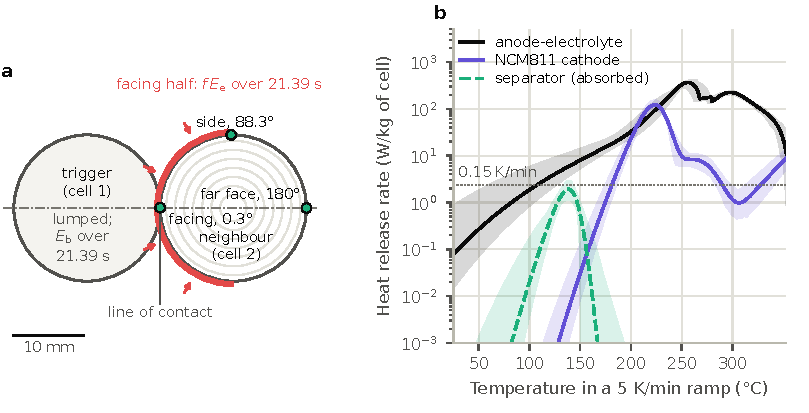
\includegraphics[width=\textwidth]{figures/fig1.pdf}
\caption{The two cells and the kinetics. (a) Cross-section at mid-length. The trigger (cell~1, one temperature) releases its body energy $\Eb$ over 21.39~s; the neighbour (cell~2) is solved as one temperature and as a resolved half model (symmetry plane dash-dotted), the cans touching along the line of contact. From Stage~8 a fraction $f$ of the ejected energy $\Ee$ enters through the half of the neighbour's can facing the trigger (red). The three nodes at mid-length bracket the thermocouple's unreported angle. (b) Heat release rate of each submodel of the kinetics in a 5~K\,min$^{-1}$ ramp from 25\degC, per kilogram of cell: the posterior mean (lines) and the 2.5 to 97.5\,\% band over the 200 posterior draws; the separator's melting absorbs heat, and its magnitude is shown. Dotted: a self-heating rate of 0.15~K\,min$^{-1}$ at the cell's specific heat. The schematic and every figure were drawn by scripts, written with a generative AI model (Section~\ref{sec:prereg}), from the results files.}
\label{fig:geometry}
\end{figure}

\subsection{The kinetics, their posterior and the SEI}
\label{sec:kinetics}

The decomposition kinetics are the Bayesian chemical reaction neural network of Koenig, Zhao and Deng~\cite{Koenig2025}, trained on calorimetry of NCM811 and graphite: seven anode, electrolyte, SEI and binder reactions, three cathode reactions and the separator's melting, each an Arrhenius rate with learned orders, whose heat enters per unit cell mass at the reactant mass fractions of the source's reference cell. The model is the mean of each parameter over the source's posterior particles; its DSC curves reproduce the source's at 5~K\,min$^{-1}$, and Fig.~\ref{fig:geometry}b shows each submodel's heat release in such a ramp. The posterior enters as 200 joint draws, each one particle of each submodel's file taken independently with replacement. The SEI starts fresh, at the source's initial amount; the aged SEI of Stage~7 starts at none. A node starts to self-heat when its reaction heat alone heats it at 0.15~K\,min$^{-1}$, and it propagates in the model when it reaches 255.7\degC, the lower edge of the source's internal-short band~\cite{Koenig2025}. An emulation of the source's accelerating-rate test gives a runaway onset of 179.3\degC, inside the source's band of 169.0 to 198.0\degC; its internal-short temperature at the stated trigger rate is 199.8\degC, below the source's band, a mismatch this study does not resolve.

\subsection{The tests, the triggers and the ejected energy}
\label{sec:tests}

Fransson et al.~\cite{Fransson2024} ran sixteen two-cell propagation tests of LG M50 cells in direct contact, joined by welded tabs, eight in parallel and eight in series, the trigger penetrated by a nail and a thermocouple fastened at the middle of each cell's surface (Table~\ref{tab:tests}; tests are named here without the prefix M50). Nine propagated, at 147 to 342~s from the trigger's runaway. The neighbours of five of the seven that did not peaked at 71 to 133\degC; the other two report 626 and 808\degC, which may not be the neighbour's surface, and are read as exploratory. The model's clock starts with the trigger's release, read as the start of its runaway. Each test gets its own trigger: the body energy $\Eb$ that puts cell~1's peak at the test's measured trigger maximum at the central contact, released over 21.39~s, the mean of the two trigger rise times the paper's supplement gives~\cite{Fransson2024}. $\Eb$ runs from 9.0~kJ (PT\_Exp1, 164\degC) to 54.3~kJ (SP\_Exp3, 832\degC). The energy a trigger ejects as vent gas, ejecta and flame is $\Ee=r\,\Eb$, with $r=3.105$ the median ejected-to-body ratio of the ten LG M50 nail tests of the Battery Failure Databank~\cite{Finegan2024}, bracketed by their smallest and largest, 2.218 and 4.156; $\Ee$ runs from 27.9 to 168.6~kJ.

\begin{table}[t]
\centering
\footnotesize
\setlength{\tabcolsep}{2.7pt}
\caption{The sixteen two-cell LG M50 tests of Fransson et al.~\cite{fransson2024exploring} (their Tables 3 and 4), with the trigger's body energy $E_\mathrm{b}$ that puts the model's trigger at the measured peak at the central contact over 21.39~s, and the ejected energy $E_\mathrm{e}=3.105\,E_\mathrm{b}$. Times run from the trigger's runaway to the neighbour's onset. The two maxima marked $^{a}$ may not be the neighbour's surface and are read as exploratory. Category, Fransson et al.'s failure category: 1, the trigger's nail-penetration failure; 2, failure in the propagating cell; 4, sidewall rupture of the trigger; c.m., ``cell movement'' in the X-ray camera's field of view, given in place of a category; a dash, none given.}
\label{tab:tests}
\begin{tabular}{llrrrlrrc}
\toprule
Test & Connection & \multicolumn{1}{c}{Trigger} & \multicolumn{1}{c}{$E_\mathrm{b}$} & \multicolumn{1}{c}{$E_\mathrm{e}$} & Propagated & \multicolumn{1}{c}{Time} & \multicolumn{1}{c}{Neighbour} & Category \\
 & & peak (\textdegree C) & (kJ) & (kJ) & & (s) & max. (\textdegree C) & \\
\midrule
PT\_Exp1 & parallel & 164 & 9.0 & 27.9 & no &  & 71 & c.m. \\
PT\_Exp2 & parallel & 679 & 43.4 & 134.8 & no &  & 808$^{a}$ & 1 \\
PT\_Exp3 & parallel & 507 & 31.6 & 98.1 & no &  & 118 & 4 \\
PT\_Exp4 & parallel & 630 & 40.0 & 124.2 & yes & 272 & 607 & 4 \\
PP\_Exp1 & parallel & 787 & 51.1 & 158.6 & yes & 152 & 381 & c.m. \\
PP\_Exp2 & parallel & 644 & 41.0 & 127.2 & yes & 147 & 699 & 2 \\
PP\_Exp3 & parallel & 686 & 43.9 & 136.3 & no &  & 105 & -- \\
PP\_Exp4 & parallel & 728 & 46.9 & 145.5 & yes & 275 & 523 & 2 \\
\midrule
ST\_Exp1 & series & 788 & 51.1 & 158.7 & no &  & 128 & 1 \\
ST\_Exp2 & series & 723 & 46.5 & 144.3 & no &  & 133 & 4 \\
ST\_Exp3 & series & 282 & 16.6 & 51.7 & yes & 177 & 763 & 1 \\
ST\_Exp4 & series & 756 & 48.8 & 151.6 & yes & 342 & 733 & 1 \\
SP\_Exp1 & series & 728 & 46.8 & 145.4 & yes & 223 & 546 & 2 \\
SP\_Exp2 & series & 755 & 48.7 & 151.3 & yes & 149 & 698 & c.m. \\
SP\_Exp3 & series & 832 & 54.3 & 168.6 & yes & 210 & 420 & c.m. \\
SP\_Exp4 & series & 625 & 39.6 & 123.0 & no &  & 626$^{a}$ & -- \\
\bottomrule
\end{tabular}
\end{table}


\subsection{The criteria}
\label{sec:criteria}

Stage~7 read seven candidate ignition criteria from each run with no new physics: the hot spot reaches 255.7\degC{} (C1); the lumped neighbour reaches 255.7\degC{} (C2); the lumped neighbour reaches 150\degC, the paper's criterion (C3); the separator's melting, 138.5\degC, at the hot spot (C4) or in the lumped neighbour (C5); and C1 and C4 with the aged SEI (C6, C7). A criterion predicts propagation when it is met within 900~s, and its time when it is met. From Stage~8 on, C1 is the local criterion and C2 the whole-cell clock. Stage~7 also ran the internal short as an event: the neighbour's stored 65.52~kJ released over 21.39~s from its separator's melting, a modelling choice.

\subsection{The delivery and its brackets}
\label{sec:delivery}

From Stage~8 on, a fraction $f$ of the trigger's ejected energy reaches the neighbour as a triangular pulse over 21.39~s from the start of the release, a uniform flux through the half of the can facing the trigger (Fig.~\ref{fig:geometry}a); the lumped neighbour receives the same energy. $f$ is a model quantity, the fraction a conduction-and-delivery model needs, not a measurement of what reached the neighbour. The brackets, run as sensitivities, are a delivery over 10 or 60~s, the quarter of the facing half nearest the cap, the ratio's two ends, Joule heat of 5 or 20\,\% of the stored energy in the parallel tests, the gas layer between the roll and the can of Hoelle, Zimmermann and Hinrichsen~\cite{Hoelle2023}, and, in Stage~9, a constant power over 120, 240 or 360~s.

\subsection{The readings: $\fs$, $\ft$ and $\fmax$}
\label{sec:readings}

$\fs$, a test's threshold for a criterion, is the bracket $(\mathrm{lo},\mathrm{hi}]$ of the smallest fraction at which the model meets it, from $f=0$ through 0.1, 0.2 and 0.3, then 0.5 and 1, halving to a width of at most 0.02; it is 0 where the run with no delivery already meets it, and its value is the bracket's midpoint. A propagated test's outcome is reproduced at $\fs$ and above, a non-propagated test's below it. Stage~9 read each test's own measurement as a fraction: $\ft$, at which a criterion is met at the measured time, for the propagated tests (bisection to 0.005, or a run within 10~s), and $\fmax$, at which the far face peaks at the measured maximum, for the others (bisection to 0.005, or a peak within 5~K, over 900~s). A propagated test is read by its time only and a non-propagated test by its peak only, because after ignition the model's temperatures are not comparable with the measured maxima.

\subsection{The history and the thermocouple's angle}
\label{sec:history}

No raw series of the tests is published. Stage~10 read the one published history of a neighbour before propagation, PT\_Exp4's, and the one of a test that did not propagate, PP\_Exp3's, out of the vector paths of the supplement's Figure~10~\cite{Fransson2024}, twice by separate code, to 2.47 and 2.46~K and 0.45~s, and checked them against the page's pixels. Each model history at the far face was compared with PT\_Exp4's record by the root mean square of the difference over 0 to 271.5~s, the onset the figure marks. The paper places the thermocouple at the middle of the surface at an angle it does not give, so three nodes at mid-length bracket it: facing the trigger (0.33\textdegree{} from the line of contact), at the side (88.28\textdegree) and at the far face (180\textdegree).

\subsection{Held-out scores and ranks}
\label{sec:heldout}

Each predictor ($\fs$(C1), $\fs$(C2), and Stage~9's fraction, $\ft$(C2) or $\fmax$) was fitted on the eight series tests and scored on the eight parallel ones, and the other way round: a penalised (Firth) logistic regression of the outcome on the predictor, against one probability for every test, $(k+0.5)/(n+1)$, by the mean log score and the Brier score, with permutation $p$-values and bands from 10,000 relabellings of the outcomes. A predictor counted as better if it beat the constant by 0.1 in the mean log score, a margin registered before the scoring. Spearman's correlation ranked each quantity against the outcomes and the measured times.

\subsection{The bands of Stage 11}
\label{sec:draws}

Stage~11 asked how much of the central numbers the kinetic and the thermal uncertainty could account for. Four kinetic draws were chosen by rank, before its predictions, from Stage~3's 200 draws ranked by the hottest node's onset in the headline passive case (ranks 5, 50, 151 and 196), and four thermal draws from Stage~3's 30 Latin hypercube draws of the roll's published properties~\cite{ORegan2022,Chen2020}: the smallest and largest conductivity across the layers and the smallest and largest heat capacity. A thermal draw sets the neighbour's roll; the trigger's history stays central. For four tests (the smallest and largest trigger energy, and the two tied nearest the median) $\fs$(C1) and $\fs$(C2) were searched under each draw from Stage~8's bracket; the far face at $f=0$ was run under each thermal draw and at the low and high contacts for the five low-maximum tests; and the nine propagated tests were run at their $\ft$(C2) under each kinetic draw. Its bands are over four draws a side, not over the posterior; the full-posterior quantity the study has is Stage~3's band of the onset lead over 200 draws.

\subsection{Pre-registration and verification}
\label{sec:prereg}

Each stage's predictions file was committed and pushed before any of its runs; its commit, push time and the hash of its run list are in the repository's record~\cite{Satte2026repo}, and the files were not changed afterwards. Through Stage~10 the study registered 64 predictions, of which 32 failed; Stage~11 registered six more (Table~\ref{tab:predictions}; every prediction, its expectation and its verdict in the supplement). Every stage closed the energy account of every run (the largest residual $2\times10^{-11}$ of the heat taken in), halved the mesh spacing and the step limits on a run near its threshold (the hot spot's peak rise moved by at most 0.52\,\%), recomputed its registered numbers by separate code, and had every registered number and verdict read again by a separate agent before its texts were written. The code was written, run and checked with the help of a generative AI model under the author's direction (see the declaration below).

\section{Results}
\label{sec:results}

\subsection{The resolved and the lumped neighbour disagree on when the chemistry starts, and the kinetics set both}
\label{sec:res-onset}

Every history that self-heats first does so at 108.4\degC, by decomposition of the fresh SEI (Fig.~\ref{fig:geometry}b). With copper busbars (500~mW\,K$^{-1}$) and the largest Databank energy, 33.2~kJ, the resolved neighbour's hottest node starts 23.4 and 26.4~s before the lumped node (10 and 30~s releases). Over the 200 posterior draws the lumped node never starts first in any of 42 cases, and at the headline case the lead runs from 15.4 to 58.9~s (2.5 to 97.5\,\%), with two modes (Fig.~\ref{fig:lead}a). Over the published spread of the roll's conductivity and heat capacity the hottest node's onset varies 0.027 times as much as over the kinetic posterior, and the lumped node's 0.11 times: the kinetics set both onsets, and the anode-electrolyte submodel, which holds the SEI, carries 0.997 of the lead's variance. Fed back, the reaction heat moves the hot spot's entry into the internal-short band by less than 0.01~s: conduction from the busbar sets it.

\begin{figure}[t]
\centering
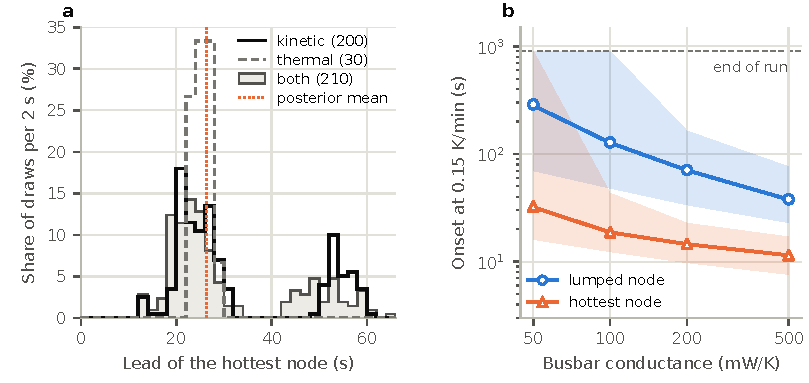
\includegraphics[width=\textwidth]{figures/fig2.pdf}
\caption{The onset in the published two-cell geometry (cells 2~mm apart, busbars), 33.2~kJ released over 30~s. (a) The hottest node's lead over the lumped node (the lumped node's onset at 0.15~K\,min$^{-1}$ less the hottest node's) at 500~mW\,K$^{-1}$: over the 200 kinetic draws at the central thermal properties, the 30 thermal draws at the posterior-mean kinetics and the 210 combined pairs; dotted, the posterior mean. (b) Onset against the busbar conductance: median (lines) and 2.5 to 97.5\,\% band over the 200 kinetic draws, and the posterior mean (markers). A band that reaches the end of the run holds draws in which that node does not start within 900~s.}
\label{fig:lead}
\end{figure}

\subsection{Conduction and radiation alone do not ignite the neighbour}
\label{sec:res-conduction}

In none of 5,248 runs with the cans in contact, across the contact, tab, energy and ambient brackets and the 200 draws, does either neighbour reach 255.7\degC{} within 900~s; the hot spot peaks at most at 226.7\degC{} and the lumped neighbour at 180.6\degC. With the trigger's release matched to the tests' durations the trigger peaks at 526 to 537\degC, inside the measured 164 to 832\degC, and neither neighbour ignites in 442 runs with the draws (Fig.~\ref{fig:passive}b). Only the Databank's total energy with the ejecta, 107~kJ, which puts the trigger at 1,424 to 1,494\degC, takes the hot spot to 255.7\degC, in every run at 8 to 17~s. By the paper's 150\degC{} criterion only the lumped neighbour at the central contact crosses inside the measured window (Fig.~\ref{fig:passive}a).

\begin{figure}[t]
\centering
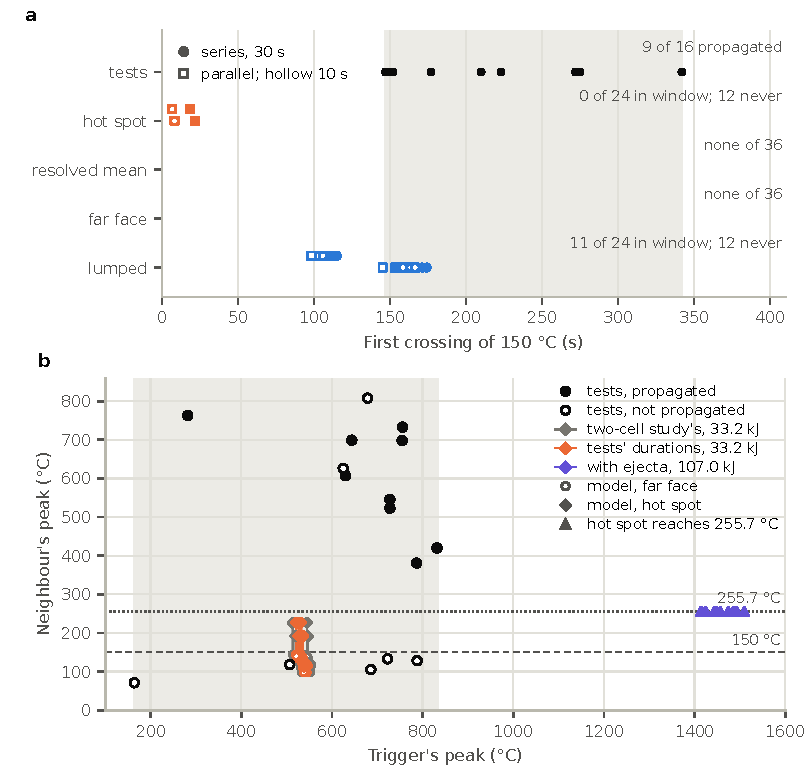
\includegraphics[width=\textwidth]{figures/fig3.pdf}
\caption{Conduction and radiation only, the cans in contact. (a) First crossing of 150\degC, the paper's criterion, by four clocks of the neighbour in 36 runs at the posterior-mean kinetics (three contacts, three tab conductances, releases of 10 and 30~s, both connections; within a row, the low, central and high contact from the bottom), against the nine measured times (top; shaded, their range). (b) The neighbour's peak against the trigger's: the sixteen tests (black) and the model's far face (circles) and hot spot (diamonds), joined per run, for the two-cell study's trigger, the trigger released over the tests' durations, and the Databank's total energy with the ejecta, 107.0~kJ; a run whose hot spot reaches 255.7\degC{} ends there (triangles). Shaded: the range of the measured trigger peaks.}
\label{fig:passive}
\end{figure}

\subsection{The local criterion predicts which tests propagate, but never when; the whole-cell clock predicts when, but rarely whether}
\label{sec:res-criteria}

With each test's own trigger, the hot spot at 255.7\degC{} (C1) predicts eight tests, six of them hits, and gets 11 of 16 outcomes right, more than any other criterion (Fig.~\ref{fig:criteria}); every hit comes 130 to 323~s before the measured time, because the hot spot crosses by 21.7~s. The lumped neighbour at 255.7\degC{} (C2) predicts two tests, both hits; at 150\degC{} (C3) and at the separator's melting (C4, C5) the criteria predict fourteen and get nine right. The aged SEI changes no hot-spot verdict. The internal short as an event overshoots: it takes the hot spot to 1,504 to 1,584\degC, about twice the hottest propagating neighbour, 763\degC. Near its own threshold the whole-cell clock has the induction the tests show and the hot spot none (Fig.~\ref{fig:fractions}a): with the 21.39~s delivery, C2 reproduces six of the nine measured times within 10~s, at $\ft$(C2) of 0.0016 to 0.047 (0.27 to 5.96~kJ), while C1, wherever it crosses, does so by 21.1~s and reproduces none.

\begin{figure}[t]
\centering
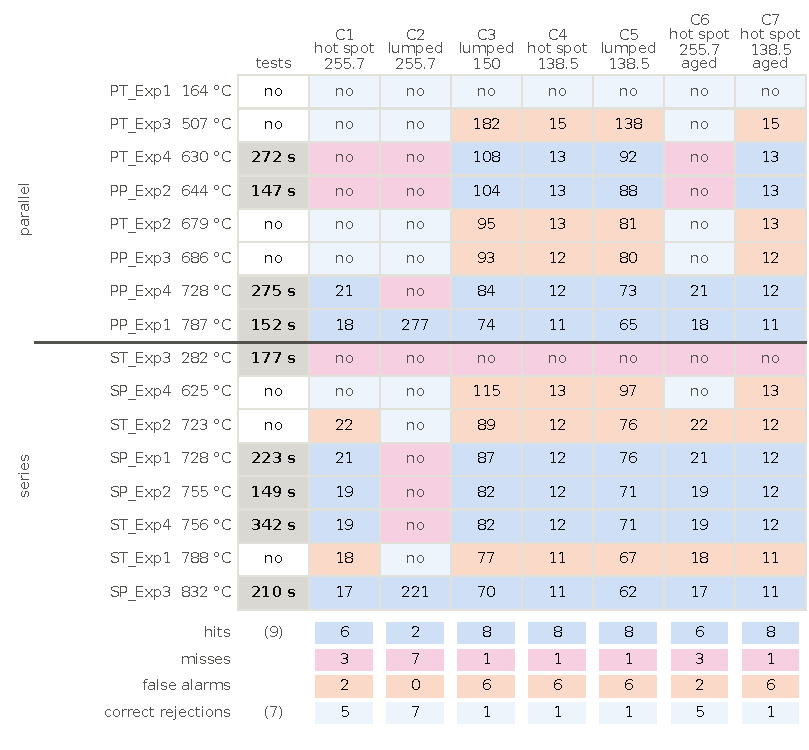
\includegraphics[width=\textwidth]{figures/fig4.pdf}
\caption{The sixteen tests (rows; parallel above, series below, each in order of the trigger's measured peak) against the seven criteria at the central contact, each test with its own trigger: the time in seconds, from the start of the trigger's release, at which the criterion is met, or no. Shading: a hit or a correct rejection (blue tints), a false alarm (orange), a miss (pink). The first column gives the measured outcome and time; the bottom rows count the classes.}
\label{fig:criteria}
\end{figure}

\subsection{A delivered part of the ejected energy is needed, and what each test needs varies 42- to 208-fold}
\label{sec:res-fraction}

For the hot spot, $\fs$(C1) is 0 in eight tests and at most 0.1625 in all; for the lumped neighbour, $\fs$(C2) is at most 0.05 in thirteen tests and at most 0.4625 in all, both highest in PT\_Exp1, the smallest trigger (Fig.~\ref{fig:thresholds}a, Table~\ref{tab:fractions}). The two groups overlap: the nine propagated tests need $\fs$(C1) of 0 to 0.0875 and the seven that did not reach it at 0 to 0.1625 ($\fs$(C2): 0 to 0.2375 against 0 to 0.4625), so no single fraction reproduces the sixteen outcomes. At a common fraction of 0.1, 0.2 or 0.3 every clock crosses by 88.3~s after the release and every hit comes 126 to 339~s early (Fig.~\ref{fig:thresholds}b). Read from each test's own time or peak, the fraction the lumped neighbour's criterion needs varies 47.6-fold between tests with the 21.39~s delivery and 42.2- to 208.1-fold with the constant powers, and the propagated and non-propagated tests overlap in it too (Fig.~\ref{fig:fractions}b). Among the brackets, the ratio's ends scale every $\fs$ by 0.75 to 1.40; with the gas layer of Hoelle et al.~\cite{Hoelle2023} the hot spot of the three tests nearest the median trigger stays below 255.7\degC{} at $f=0.2$ (192.4 to 196.5\degC), where without it it crosses at 3.5 to 3.7~s.

\begin{table}[t]
\centering
\footnotesize
\caption{The fractions of the ejected energy each test needs in the model. $f^*$(C1) and $f^*$(C2): the threshold bracket $(\mathrm{lo},\mathrm{hi}]$ at which the hot spot (C1) or the lumped neighbour (C2) reaches 255.7\textdegree C with the 21.39~s delivery, 0 where no delivery is needed. $f_\mathrm{t}$(C2): the fraction at which the lumped neighbour's crossing comes at the measured time ($^{b}$ the search ended at the threshold, its bracket given). $f_\mathrm{max}$: the fraction at which the far face peaks at the measured maximum ($^{a}$ exploratory). The last three columns give Stage 11's ranges where it ran: $f^*$(C2) over the posterior mean and the eight draws; the far face's peak at $f=0$ less the measured maximum over the central case, the four thermal draws and the two contact brackets; and the lumped neighbour's crossing at $f_\mathrm{t}$(C2) under the four kinetic draws, with the number that do not cross within 900~s.}
\label{tab:fractions}
\begin{tabular}{lllllll}
\toprule
Test & $f^*$(C1) & $f^*$(C2) & $f_\mathrm{t}$(C2) or $f_\mathrm{max}$ & $f^*$(C2), & Far face at & C2 crossing, \\
 & & & & 8 draws & $f=0$ (K) & kinetic (s) \\
\midrule
PT\_Exp1 & (0.15, 0.1625] & (0.45, 0.4625] & 0.075 &  &  &  \\
PT\_Exp2 & (0, 0.0125] & (0.0125, 0.025] & 0.5625$^{a}$ &  &  &  \\
PT\_Exp3 & (0.025, 0.0375] & (0.075, 0.0875] & 0 &  &  &  \\
PT\_Exp4 & (0, 0.0125] & (0.0375, 0.05] & (0.0375, 0.040625]$^{b}$ &  &  &  \\
PP\_Exp1 & 0 & 0 & 0.01875 &  &  &  \\
PP\_Exp2 & (0, 0.0125] & (0.025, 0.0375] & 0.046875 &  &  &  \\
PP\_Exp3 & (0, 0.0125] & (0.0125, 0.025] & 0 &  &  &  \\
PP\_Exp4 & 0 & (0, 0.0125] & 0.0125 &  &  &  \\
ST\_Exp1 & 0 & (0, 0.0125] & 0 &  &  &  \\
ST\_Exp2 & 0 & (0.0125, 0.025] & 0 &  &  &  \\
ST\_Exp3 & (0.075, 0.0875] & (0.225, 0.2375] & (0.23125, 0.234375]$^{b}$ &  &  &  \\
ST\_Exp4 & 0 & (0, 0.0125] & (0.00625, 0.009375]$^{b}$ &  &  &  \\
SP\_Exp1 & 0 & (0.0125, 0.025] & 0.01875 &  &  &  \\
SP\_Exp2 & 0 & (0, 0.0125] & 0.025 &  &  &  \\
SP\_Exp3 & 0 & 0 & 0.0016 &  &  &  \\
SP\_Exp4 & (0, 0.0125] & (0.0375, 0.05] & 0.265625$^{a}$ &  &  &  \\
\bottomrule
\end{tabular}
\end{table}


\begin{figure}[t]
\centering
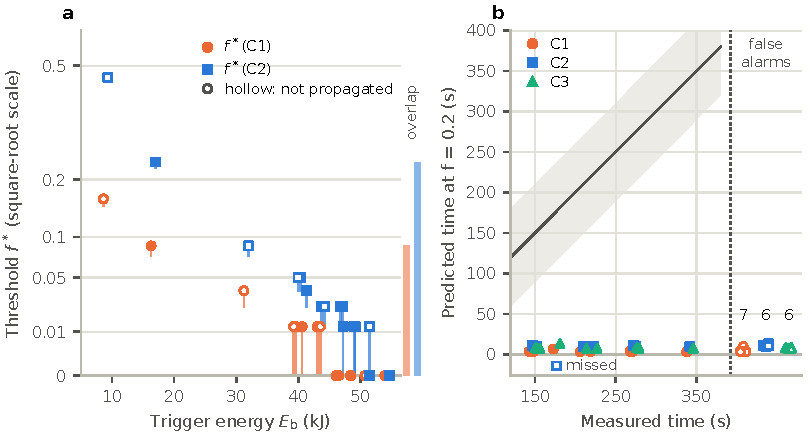
\includegraphics[width=\textwidth]{figures/fig5.pdf}
\caption{The delivered fraction the outcomes require. (a) $\fs$(C1) (circles) and $\fs$(C2) (squares) of the sixteen tests against the trigger's body energy, each as its bracket from the largest fraction that does not meet the criterion to the smallest that does (marker); filled, propagated; hollow, not. The bars at the right mark where the ranges of the two groups overlap. Square-root scale. (b) At a fraction common to every test, $f=0.2$: each criterion's predicted time against the measured time for the propagated tests it predicts (a missed test below the axis) and, at the right, the predicted times of its false alarms, with their number. The line is equality, the band 60~s either side.}
\label{fig:thresholds}
\end{figure}

\subsection{Conduction alone overheats the far face in four of the five non-propagated tests}
\label{sec:res-farface}

With no delivery the far face already peaks 13.8 to 56.3~K above the measured maxima of PT\_Exp3, PP\_Exp3, ST\_Exp1 and ST\_Exp2, so their $\fmax$ is 0; PT\_Exp1, the smallest trigger, needs 0.075 (2.09~kJ) for its 71\degC. That 0.075 lies above the smallest $\ft$(C2), SP\_Exp3's 0.0016, while the four zeros lie below every $\ft$: the fractions read from the times and the peaks do not separate the groups either. The thermocouple's angle does not remove the overshoot: at 88.3\textdegree{} or facing the trigger the four low maxima still need no delivery (overshoot 13.8 to 159.9~K), and only facing the trigger, with all five at 0, do the fractions separate the groups. In PP\_Exp3's published record, the far face with no delivery lies 41.7~K above the measurement on average over 500~s (peaks 161.3 against 102.0\degC).

\begin{figure}[t]
\centering
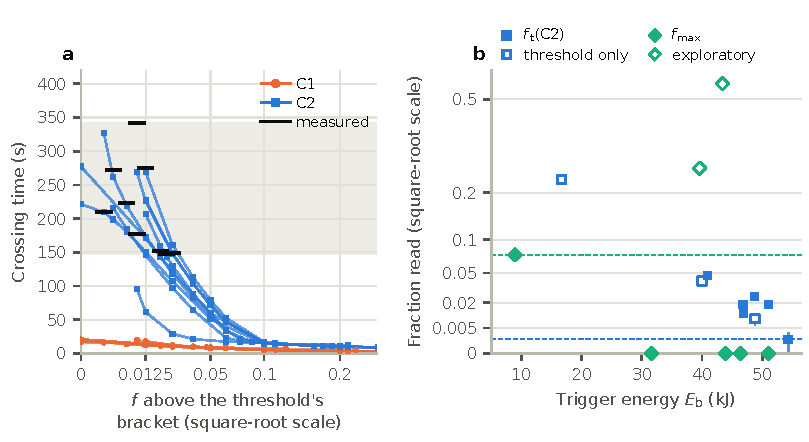
\includegraphics[width=\textwidth]{figures/fig6.pdf}
\caption{The fractions read from each test's own measurement. (a) With the 21.39~s delivery, each propagated test's crossing time against the fraction above the lower end of its threshold bracket, for the hot spot (C1) and the lumped neighbour (C2), one line per test and criterion; black bars, the measured times; shaded, their range. Square-root scale. (b) Against the trigger's energy: $\ft$(C2) for the propagated tests (hollow where the search ended at the threshold, shown with its bracket) and $\fmax$ at the far face for the others (hollow, the two exploratory maxima). Dashed: the largest registered $\fmax$ and the smallest $\ft$(C2).}
\label{fig:fractions}
\end{figure}

\subsection{The one published neighbour history follows a short delivery near its threshold, and no long one}
\label{sec:res-history}

PT\_Exp4's thermocouple reaches 141.0\degC{} by 45~s and rises steadily to 197.3\degC{} at the onset, 271.5~s (Fig.~\ref{fig:history}a). At the far face, the 21.39~s delivery at the two ends of its C2 bracket ($f=0.0375$ and 0.040625) lies 16.3 and 16.8~K from the record (root mean square to the onset), the constant powers at their $\ft$ 36.7 to 37.2~K, and no delivery 47.4~K. The difference comes from the first 100~s, the record's rise to 141\degC{} by 45~s, which only the short delivery follows; after 100~s the short and the long C2 readings lie 8.8 to 12.0~K from the record, and none has its last rise. The record's first 8.5~s, a spike to 102\degC, is read as the thermocouple's exposure at the trigger's runaway rather than the can's temperature; it holds 41.2\,\% of the short delivery's squared difference. One test's history decides between the readings for that test only.

\subsection{Held out, nothing the model yields beats one probability for every test}
\label{sec:res-heldout}

Fitted on one connection and scored on the other, no predictor beats one probability for every test by the registered margin of 0.1 in the mean log score; the largest gain is 0.062, Stage~9's fraction fitted on the series tests, and the permutation $p$-values run from 0.23 to 0.75 (Brier score, 0.20 to 0.75) (Fig.~\ref{fig:history}b). No model quantity ranks with the outcomes or the times ($p$ at least 0.13), while $\fs$(C1) and $\fs$(C2) rank with the trigger's energy ($\rho=-0.92$ and $-0.97$): the thresholds mostly restate the trigger. The sixteen tests cannot adjudicate between these models.

\begin{figure}[t]
\centering
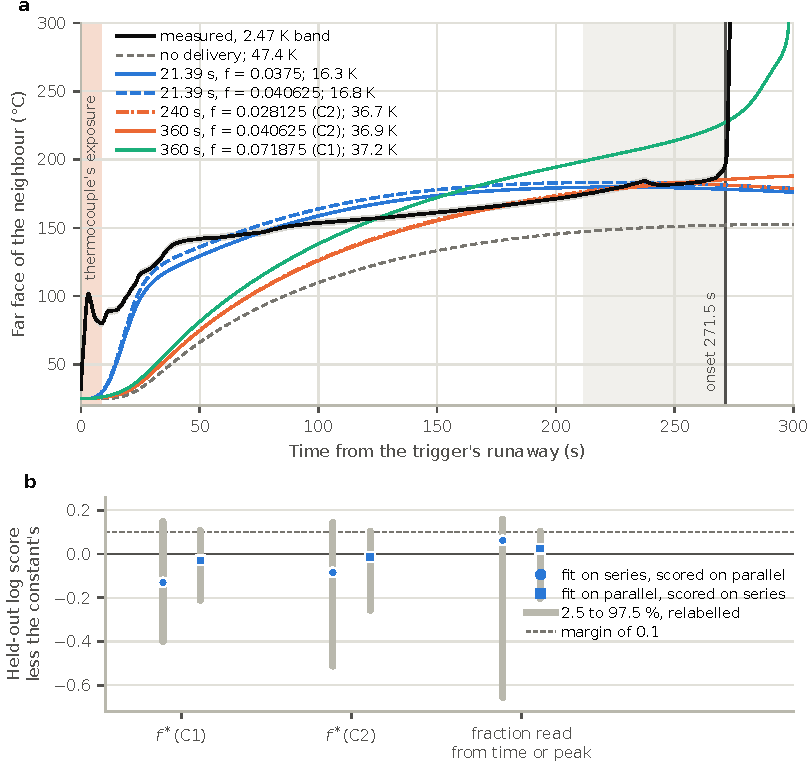
\includegraphics[width=\textwidth]{figures/fig7.pdf}
\caption{(a) PT\_Exp4's measured thermocouple record (black; band, its 2.47~K reading uncertainty) and the model's far face at the central contact under the readings Stage~9 found for that test, each with its root mean square difference from the record up to the onset, 271.5~s (vertical line). Shaded at the left, the record's first 8.5~s, a spike read as the thermocouple's exposure at the trigger's runaway, not the can; at the right, the last 60~s before the onset. (b) Held out: the mean log score of the logistic fit in each predictor less that of one probability for every test, fitted on one connection and scored on the other (markers), with the 2.5 to 97.5\,\% band over 10,000 relabellings of the outcomes. Dashed: the registered margin of 0.1.}
\label{fig:history}
\end{figure}

\subsection{How much of this the kinetic and thermal uncertainty could account for}
\label{sec:res-bands}

\PH{Stage 11 paragraph, written after its runs and the independent read}

\subsection{The predictions that failed, and what each failure taught}
\label{sec:res-failed}

\PH{failed predictions, with Table 4}

\begin{table}[t]
\centering
\footnotesize
\caption{The predictions by stage: committed before the stage's runs, held, failed, and of the failures those foreseen, which the predictions file had recorded before the runs as expected to fail, as already fixed by earlier records or an energy balance, or as failing under a condition it named that then held. The stages' own texts label 17 of the 21 through Stage 10 so (Supplement S2). Every prediction, its expectation and its verdict are in the supplement.}
\label{tab:predictions}
\begin{tabular}{p{0.44\textwidth}rrrr}
\toprule
Stage & Committed & Held & Failed & Foreseen \\
\midrule
1 and 2: passive and reactive onset & 7 & 6 & 1 & 0 \\
3: onset over the posterior and thermal draws & 6 & 3 & 3 & 2 \\
4: which submodel sets the lead & 5 & 4 & 1 & 0 \\
5: neighbours against the tests & 7 & 1 & 6 & 0 \\
6: the paper's 150\textdegree C criterion; matched trigger & 7 & 1 & 6 & 6 \\
7: seven criteria, test by test & 8 & 3 & 5 & 5 \\
8: the delivered fraction $f^*$ & 8 & 5 & 3 & 3 \\
9: fractions from times and peaks & 8 & 5 & 3 & 3 \\
10: one history; held-out scores & 8 & 4 & 4 & 2 \\
\midrule
Stages 1 to 10 & 64 & 32 & 32 & 21 \\
\midrule
11: bands under the draws & 6 & 2 & 4 & 1 \\
12: the trigger held to the calorimetry & 4 & 4 & 0 & 0 \\
\midrule
All stages & 74 & 38 & 36 & 22 \\
\bottomrule
\end{tabular}
\end{table}


\section{Discussion}
\label{sec:discussion}

\PH{discussion, written with the verified references}

\section{Conclusions}
\label{sec:conclusions}

\PH{conclusions, written last}

\section*{Declarations}

\paragraph{Funding} This research did not receive any specific grant from funding agencies in the public, commercial, or not-for-profit sectors.

\paragraph{Declaration of competing interest} The author declares no known competing financial interests or personal relationships that could have appeared to influence the work reported in this paper.

\paragraph{Data and code availability} The code, inputs, run records, checks and decisions of every stage are archived at Zenodo, \url{https://doi.org/10.5281/zenodo.23279455} (all versions; this paper uses version 1.7.0), and in the repository \url{https://github.com/siddharth161204-wq/m50-neighbour-onset-kinetics}~\cite{Satte2026repo}. The two-cell geometry is archived at \url{https://doi.org/10.5281/zenodo.23253738}~\cite{Satte2026twocell}.

\paragraph{CRediT authorship contribution statement} \textbf{Siddharth Satte:} Conceptualization, Methodology, Software, Validation, Formal analysis, Investigation, Data curation, Writing~-- original draft, Writing~-- review \& editing, Visualization, Project administration.

\paragraph{Acknowledgements} The measured tests are those of Fransson et al.~\cite{Fransson2024}, published under CC~BY~4.0. The kinetic posterior files are the supplementary data of Koenig, Zhao and Deng~\cite{Koenig2025}. The Battery Failure Databank is provided by the U.S. Department of Energy's National Renewable Energy Laboratory, operated by Alliance for Sustainable Energy, LLC (DOE/NREL/ALLIANCE)~\cite{Finegan2024}.

\paragraph{Declaration of generative AI and AI-assisted technologies in the manuscript preparation process} \PH{drafted for the author's approval}

%BODY-END

\bibliographystyle{elsarticle-num}
\bibliography{references}

\end{document}
